%% Template for EU deliverable, using the deliverable.sty style file

\documentclass[12pt,a4paper,twoside]{article}

%% common package
\usepackage[headers]{deliverable}
\usepackage{xspace}
\usepackage{verbatim}
\usepackage[usenames]{color}
\usepackage{listings}
\usepackage[usenames,dvipsnames,table]{xcolor}
\usepackage[pdftex,dvips]{graphicx}
\usepackage{url}
\usepackage{array}

\usepackage{IEEEtrantools}
%%

%%insert here other packages needed by sections

%%

%%%%%%%%%%%%%%%%%%%%%%%%%%%%%%%%%%%%%%%%%%%%%%%%%%%%%%%%%%%%%%%%%%%%%%%%%%%%%%
%%% Titlepage
%%%%%%%%%%%%%%%%%%%%%%%%%%%%%%%%%%%%%%%%%%%%%%%%%%%%%%%%%%%%%%%%%%%%%%%%%%%%%%

% declaration of variables used in style
\deliverableDocnumber{D3.3}
\deliverableTitle{Local solver in compliant and unforeseen cases}

\deliverableAuthor{Vincent Padois$^{1,2}$, Daniele Pucci$^{3}$}
\deliverableResponsiblePartner{UPMC}
\deliverableAffiliation{% Insert here authors affiliations
 $^1$ Sorbonne Universit\'es, UPMC Paris 06, UMR 7222, Institut des Syst\`emes Intelligents et de Robotique (ISIR), F-75005, Paris, France.
 
 $^2$ CNRS, UMR 7222, Institut des Syst\`emes Intelligents et de Robotique (ISIR), F-75005, Paris, France.
 
 $^3$ Istituto Italiano di Tecnologia (IIT) Via Morego 30, Genoa, Italy.
}


\deliverableCoordinator{Vincent Padois}
\deliverableActivityNumber{n} %% n=1,..,10
\deliverableActivity{Local solver in compliant-world cases}
\deliverableDoctype{Deliverable} %% or Prototype
\deliverableClassification{Public} % or Consortium
\deliverableDistribution{Consortium} %
\deliverableStatus{Final} % Draft or Final
\deliverableDeliveryDate{28/2/2017}
\deliverableFile{D3.2.pdf} % please do not use "-" in the name
\deliverableVersion{1.0}
\deliverableDate{Feb.~28, 2017}
\deliverableYear{2016}
\deliverablePages{\pageref{LastPage}}
\deliverableChangelog{}
\deliverableProjectStartingDate{1st March 2013}
\deliverableProjectEndDate{28th February 2017}
\deliverableProjectAcronym{CoDyCo}
\deliverableProjectTitle{Whole-Body Compliant Dynamical Contacts in Cognitive Humanoids}
\deliverableContractNumber{600716}
\deliverableProjectCoordinator{Istituto Italiano di Tecnologia}
\deliverableProjectUrl{www.codyco.eu}
\deliverableFrameworkProgramme{FP7}
 
\deliverableWorkpackage{WP3}
\deliverableEditors{Vincent Padois, Daniele Pucci}
\deliverableContributors{Morteza Azzad, Mingxing Liu, Michael Mistry, Francesco Nori, Vincent Padois, Daniele Pucci, Francesco Romano, Silvio Traversaro}

\deliverableAbstract{This deliverable provides an overview of the whole-body control strategies proposed within the framework of the CoDyCo project for balancing by means of  contacts and unforeseen robot interactions. We first recall the general structure of the whole-body controller used in the CoDyCo project. This controller is written as a quadratic multi-objective optimization problem under linear constraints, and priorities between the control objectives can be dealt with through strict or soft hierarchy. The control architecture is then modified in order to deal with unforeseen cases. More precisely, we assume that a user can interact with the robot at specific locations, namely, the robot forearms. Then, we propose a passivity-based modification to the controller in order to take into account the robot interaction according to its desired motion. This deliverable is strongly related to Deliverable~5.5 \cite{deliverable53} which discusses the technical details and choices for the implementation of the year-4 validation scenario.}
\deliverableReviewers{}
\deliverableKeywordList{Whole-body controllers, Non-rigid contacts, Multi-contacts}

%%%%%%%%%%%%%%%%%%%%%%%%%%%%%%%%%%%%%%%%%%%%%%%%%%%%%%%%%%%%%%%%%%%%%%%%%%%%%%
%%% Sections
%%%%%%%%%%%%%%%%%%%%%%%%%%%%%%%%%%%%%%%%%%%%%%%%%%%%%%%%%%%%%%%%%%%%%%%%%%%%%%

%% constants
\newcommand{\botegoCaps}{BOTEGO}
\newcommand{\certhCaps}{CERTH}
\newcommand{\cybionCaps}{CYBION}
\newcommand{\nuigCaps}{NUIG}
\newcommand{\ubitechCaps}{UBITECH}
%%

%%%%%%%%%%%%%%%%%%%%%%%%%%%%%%%%%%%%%%%%%%%%%%%%%%%%%%%%%%%%%%%%%%%%%%%%%%%%%%
%%% Misc. by Vincent
%%%%%%%%%%%%%%%%%%%%%%%%%%%%%%%%%%%%%%%%%%%%%%%%%%%%%%%%%%%%%%%%%%%%%%%%%%%%%%
\usepackage{titlesec}
\newcommand{\sectionbreak}{}
\graphicspath{{./figure/}}
\usepackage{pdfpages}
\usepackage{caption}
\usepackage{subcaption}
\usepackage{slashbox}
\usepackage{multirow}
\usepackage{appendix}
\usepackage{amsmath} % assumes amsmath package installed
\usepackage{amssymb}  % assumes amsmath package installed
\usepackage[ruled,vlined,linesnumbered]{algorithm2e}
\usepackage{mathtools}
\usepackage{graphicx}
\usepackage{hyperref}
\hypersetup{
    bookmarks=true,         % show bookmarks bar?
    unicode=false,          % non-Latin characters in Acrobat’s bookmarks
    pdftoolbar=true,        % show Acrobat’s toolbar?
    pdfmenubar=true,        % show Acrobat’s menu?
    pdffitwindow=false,     % window fit to page when opened
    pdfstartview={FitH},    % fits the width of the page to the window
    pdftitle={D32.pdf},    % title
    pdfauthor={Vincent Padois},     % author
    pdfsubject={Local solver in compliant-world cases},   % subject of the document
    pdfcreator={Vincent Padois},   % creator of the document
    pdfproducer={Vincent Padois}, % producer of the document
    pdfkeywords= {Whole-body controllers, Non-rigid contacts, Multi-contacts}, % list of keywords
    pdfnewwindow=true,      % links in new window
    colorlinks=true,       % false: boxed links; true: colored links
    linkcolor=black,          % color of internal links (change box color with linkbordercolor)
    citecolor=black,        % color of links to bibliography
    filecolor=black,      % color of file links
    urlcolor=black           % color of external links
}

\newcommand{\vect}[1]{\mbox{\boldmath${#1}$}}%$
\newcommand{\av}{\vect{\chi}}
\newcommand{\tens}[1]{#1}
\DeclareMathOperator*{\argmin}{argmin}

%%%%%%%%%%%%%%%%%%%%%%%%%%%%%% BEGIN DOCUMENT
\begin{document}

\deliverableMaketitle

%%TODO move to style
\newcolumntype{L}[1]{>{\raggedright\let\newline\\\arraybackslash\hspace{0pt}}m{#1}}
\newcolumntype{C}[1]{>{\centering\let\newline\\\arraybackslash\hspace{0pt}}m{#1}}
\newcolumntype{R}[1]{>{\raggedleft\let\newline\\\arraybackslash\hspace{0pt}}m{#1}}

\textbf{Document Revision History}
\begin{center}
\begin{tabular}{|C{2cm}|C{3cm}|C{5cm}|C{4cm}|}
\hline
\textbf{Version}&\textbf{Date}&\textbf{Description}&\textbf{Author}\\\hline
v.~0.1 & Jan.~19, 2016 & Initial creation of the file & Vincent Padois\\ \hline
v.~0.9 & Feb.~25, 2016 & Final version & Vincent Padois \\ \hline
v.~1.0 & Feb.~27, 2016 & Proofread version & Vincent Padois \\ \hline
\end{tabular}
\end{center}
 
 \clearpage

\newpage
\renewcommand*\contentsname{Table of Contents}
\renewcommand*\listfigurename{Index of Figures}
\tableofcontents
\newpage
\listoffigures
\newpage

%%%%%%%%%%%%%%%%%%%%%%%% Start deliverable content here.

\section{Introduction}


Under-actuated robots, such as free-floating humanoid robots, usually need to make contacts with their environments to achieve some goal directed whole-body movements. Most researches on whole-body control assume that the environment of the robot is rigid. This means that no adaptation to the environment compliance is needed for controllers. In reality, there is no completely rigid surface even if in practice we can assume a surface to be rigid if it is stiff enough (i.e. deflection is negligible). Unfortunately, many objects in human environments cannot be considered as stiff enough and their compliance has to be accounted for (e.g. a soft cushion, a sofa, a yoga carpet). Indeed, a controller that does not take into account the compliant  properties of the contact material may not be sufficient:  the compliance of
the contact has to be considered by the controller, otherwise the robot may fail to properly balance and fall over. For example, %pushing too strongly against a rigid object may result in damages to the robot or the environment; and 
pushing too weakly against a compliant object may not provide the robot with enough reaction forces to support its whole-body tasks. The problem is complex as the rigidity of the object in contact is unknown a priori to robotic controllers, which is usually the case in many scenarios.\\
 

The humanoid whole-body control problem has been addressed by different types of whole-body controllers, using analytical approaches \cite{Khatib08,Sentis10,Righetti13}, constrained quadratic programming \cite{Abe07,Liu11,Salini11,Salini13,Saab13}, or a mixture of them \cite{Stephens10,Nori15}. These controllers are either developed for rigid environments, or validated only in rigid contact scenarios.
In general, a valid set of contact forces during whole-body task control can be found by solving a multi-objective problem with a set of elementary task objectives as well as constraints, such as whole-body dynamics, friction cone constraints for non-sliding contacts, and linear complementarity conditions \cite{Muico09,Saab13,Salini11,Salini13}, which implies zero relative motions between two bodies in contact when normal contact force is non-negative. In the case of rigid contact with static environment, the linear complementarity condition implies two constraints: (i) the motion of the contact point is zero and (ii) the contact force along the normal to the contact surface is non-negative.  The zero motion constraint may not necessarily be true in the case of non-rigid contacts, since the velocities or accelerations of contact points may be non-zero, although the relative motion between the two contact points remains zero. In this case, hybrid control methods \cite{khatib87} that control forces and motions in orthogonal directions are not applicable. Therefore, the controller should take into account the dynamic relation between the contact point position and the contact force, rather than just control the contact force alone.\\ 

Such physical interaction dynamics is taken into account in impedance control \cite{Hogan85} with the idea of controlling the relation between the contact point motion and the reaction force. Traditional impedance control \cite{Hogan85,Love95,Tsumugiwa02} computes the target impedance of the robot according to the estimated impedance of the environment, which requires high quality measurement of interaction forces. In \cite{Buchli10, Yang11}, learning approaches are applied to optimize the robot impedance. Such approaches do not require interaction force sensing and can be adaptable to variable environment impedance. However, the application of such approaches in the context of humanoid balance control with non-rigid contacts is not suitable. First, these methods rely on trajectory-based learning and adaptation algorithms, whereas there is not necessarily a reference motion trajectory for each support contact in the whole-body balancing context considered here. Furthermore, they need to explore the entire state-action space if a globally optimal solution is to be found, which is impossible for high dimensional robots such as humanoids.\\

The problem of humanoid balance control with deformable contact support was addressed in \cite{Bouyarmane11b}, which proposed a posture planning approach assuming that the contact material properties are known. Compliant contacts between robots and their environments have been studied by some researchers in other areas such as grasping \cite{Xydes&Kao99} and animated characters \cite{Jain&Liu11}. However, there has not been much research efforts on balancing legged robots on compliant surfaces.\\

This deliverable provides an overview of the whole-body control strategies proposed within the framework of the CoDyCo project for balancing by means of compliant contacts. It is organized as follows. We first recall the general structure of the whole-body controller used in the CoDyCo project. This controller is written as a quadratic multi-objective optimization problem under linear constraints and priorities between the objectives can be dealt with through strict of soft hierarchy. This controller has to be modified in order to deal with compliant cases and two cases are then distinguished. In the first one, no model of the environment is assumed to be known and an adaptive force regulation task is added to the original ``rigid contact" controller in order to account for the compliance of the environment. In the second case, a contact model is supposed to be known and using that knowledge a control strategy is derived.

\section{General structure of the whole-body controller in the CoDyCo project}

Even though it is not often formulated as such, control of dynamical systems is an optimization problem. Within the framework of the CoDyCo project, the whole-body controller is written as a quadratic multi-objective optimization problem under linear constraints where priorities between the objectives can be dealt with through strict of soft hierarchy. Deliverable~3.1 \cite{deliverable31} exposes the reasons why it is preferable to express controllers in this way. The logic behind this choice can be briefly summarized in a very straightforward way:
\begin{enumerate}
\item the equation of motion and joint space to task spaces mappings can be written as equalities but they are not sufficient to describe the overall dynamics and physical behaviour of a robot.
\item Indeed, other intrinsic physical constraint have to be accounted for at the joint level as well as in Cartesian space. These constraints do not solely describe relationships between physical quantities but also limits which cannot (control input saturation) or should never be crossed in order to maintain the robot and its environment in proper working conditions.
\item Theses limits translate into inequalities.
\item Assuming a convex solution space, the optimal solution of the control problem lie at the boundary of the feasible (constraint compliant) solution space.
\item Finding the optimal solution thus boils down to finding the active constraint set, \textit{i.e.} on which boundary it lies.
\item Optimization problem solvers are designed to optimally choose this subset of constraints that should be considered when computing the optimal solution of the control problem.
\item The strong mathematical background in convex optimization is such that optimization based methods mostly outperform analytical methods attempting to heuristically activate constraints.
\end{enumerate}

\subsection{Formulation}
Based on this formulation choice, the reactive control problem aims at finding at each control instant the actuation torque minimizing $T(\mathbb{X})$, some tasks related function to minimize, given the equation of motion of the multi-body system as well as other equality and inequality constraints. This can be written
\begin{subequations}\label{eq:one task}
%\begin{eqnarray}
%\vect{\tau}^*_{t} =~\argmin \limits_{\mathbb{X}_{t}} & T(\mathbb{X}_{t}, t) \label{eq:cp obj}\\  
%\text{subject to} 
%  & \mathbf{M}(\vect{q}_{t}) \vect{\dot{\nu}}_{t}+\vect{n}(\vect{q}_{t},\vect{\nu}_{t}) = \mathbf{S}\vect{\tau}_{t}+\mathbf{J}_c(\vect{q}_{t})^\top \vect{F}_{c,{t}} \label{eq:cp dyn model}\\ 
%  & \mathbf{A}(t) \mathbb{X}_{t}   =  \vect{b}(t)  \label{eq:cp eq cons} \\
%  & \mathbf{G}(t) \mathbb{X}_{t} \leq \vect{h}(t)  \label{eq:cp ineq cons}
%\end{eqnarray}
\begin{eqnarray}
{\tau}^* =~\argmin \limits_{\mathbb{X}} & T(\mathbb{X}) \label{eq:cp obj}\\  
\text{subject to} 
  & {M}(q) {\dot{\nu}}+{C}({q},{\nu}){\nu} + G(q) = {B} {\tau} + \underbrace{\sum_{k = 1}^{n_c} {J}^\top_{\mathcal{C}_k}(q) f_k}_{J^\top(q) f} \label{eq:cp dyn model}\\ 
  & {A}(q,\nu) \mathbb{X}   =  {b}(q,\nu)  \label{eq:cp eq cons} \\
  & {D}(q,\nu) \mathbb{X} \leq {h}(q,\nu)  \label{eq:cp ineq cons}
\end{eqnarray}               
\end{subequations}
where:
\begin{itemize}
\item $\tau \in \mathbb{R}^n$ is the internal actuation torque with $n + 1$ the number of rigid bodies -- called links -- connected by $n$ actuated joints with one degree of freedom each.
\item ${q} \in \mathbb{R}^3 \times SO(3)\times \mathbb{R}^n$ is the configuration of the free-floating system. $q$ is a triplet composed of the origin and orientation of the base frame expressed in the inertial frame $\left(\prescript{\mathcal{I}}{}p_{\mathcal{B}},\prescript{\mathcal{I}}{}R_{\mathcal{B}}\right)$ and the $n$ joint angles $q_j$.
\item ${\nu} \in \mathbb{R}^{n+6}$ is the system velocity, a triplet concatenating the floating-base twist $\left (^\mathcal{I}\dot{ p}_{\mathcal{B}},^\mathcal{I}\omega_{\mathcal{B}}\right)$ and the joint velocities ${\dot{q}}_j$.
\item ${J}({q})= \left[{J}^\top _{\mathcal{C}_1}({q})~ \dots~ {J}^\top _{\mathcal{C}_k}({q}) \right]^\top$ is the contact Jacobian matrix for all $k$ contact points.
\item $f= \left[ {f}^\top_{1}~ \dots~ {f}^\top_{k}~ \right]^\top $ is the vector of external contact wrenches applied by the environment on the links.
\item $\mathbb{X} = \left(\dot{\nu}, \tau, f \right)$ gathers the dynamic variables of the multi-body system.
\item ${M} \in \mathbb{R}^{(n+6) \times (n+6)}$ is the mass matrix.
\item ${C} \in \mathbb{R}^{(n+6) \times (n+6)}$ is the Coriolis and centrifugal effects matrix.
\item ${G} \in \mathbb{R}^{n+6}$ is the gravity term.
\item $B = (0_{n\times 6} , 1_n)^\top$ is a selection matrix.
\item ${A}(q,\nu) \mathbb{X}   =  {b}(q,\nu)$ gathers kinematics constraints related to the velocity of the contact points.
\item ${D}(q,\nu) \mathbb{X} \leq {h}(q,\nu)$ gathers inequality constraints related to joint limits (position and velocity), control input saturation, contact forces (existence and friction limits) and potentially obstacle avoidance.
\end{itemize}

\subsection{Dealing with multiple objectives}

The control problem is often multi-objective and the tasks-related function $T(\mathbb{X})$ can actually be written
\begin{equation}\label{eq:multi task}
T(\mathbb{X}) = T\left(\lambda_1, T_1(\mathbb{X}), \lambda_2, T_2(\mathbb{X}), \dots, \lambda_{n_t},T_{n_t}(\mathbb{X})\right)
\end{equation}
where $T_i(\mathbb{X})$ is the $i$-th task among $n_t$ operational tasks to be achieved with $J_i(q)$ its associated task Jacobian and $\lambda_i$ its priority level. $T_i$ is generally of three types:
\begin{equation}
\begin{array}{ll}
\bullet~~\text{Operational space acceleration} & T_i={J_i}({q}){\dot{\nu}} + {\dot{J}_i}({q}_t,{\nu}){\nu} -{\ddot{x}}^{d} \\
\bullet~~\text{Joint space acceleration}       & T_i={\dot{\nu}}-{\dot{\nu}}^{d} \\
\bullet~~\text{Operational space force}        & T_i={f}_{\mathcal{C}_i}-{f}_{\mathcal{C}_i}^{d}
\end{array}
\end{equation}
where ${\ddot{x}}^{d}$, ${\dot{\nu}}^{d}$ and ${f}_{\mathcal{C}_i}^{d}$ are desired Cartesian space acceleration, configuration space acceleration and contact wrench respectively, the desired value itself being the outcome of some higher level control architecture (Proportional--Derivative--Integral regulators and/or Momentum regulators and/or Model Predicitve Controllers and/or Trajectory planners providing a feedfoward reference, \textit{etc}).\\

$T_i$ usually appears in $T$ under the form of a weighted, euclidean norm thus leading to a quadratic cost associated to each task. This quadratic form and the linearity of the constraints allows to resort to the convex optimization techniques, more particularly Linear Quadratic Programs. Then, depending of the type of retained prioritization scheme, the optimization problem \ref{eq:one task} can be solved:
\begin{enumerate}
\item at once using a single LQP and soft prioritization where $T$ is written as a weighted sum of quadratic costs and where $\lambda$s play the role of weights for each task, see \cite{Salini2011,bouyarmane2011using} for examples;
\item using a cascade of LQPs thus inducing strict prioritization between tasks (in that case $\lambda$s are used to defined a lexicographic order), see \cite{Saab13,herzog2014balancing,hierarchicalq} for examples;
\item using a representation able to convey both soft and strict prioritization, see \cite{liu-AutRob2015,liu-AutRobSI2015}.
\end{enumerate}

\subsection{Direct and two-stage whole-body control approaches}

In CoDyCo, these three types of prioritization scheme coexist and are used indifferently as they allow to produce very similar types of behaviours\footnote{A formal comparison of their intrinsic properties is out of the scope of this deliverable but would constitute a work of interest for the community}. A distinction has still to be made between two ways to approach the whole-body control problem.\\

The first, direct, approach does not separate the problem of computing the contact forces from the one of computing the joint torques. Given some task space desired acceleration (among which a center of mass one), the resolution of the control problem described by Equation~(\ref{eq:one task}) directly provides the optimal torques. The contact forces come as a by-product of the problem resolution. This approach has the very nice property of being able to account for the all constraints in a straightforward way. Its drawback is that it hides some of the essence of the balance control problem and while it may be preferable to use such a solution for practical implementation, a two-stage solution may be preferred to ease the analysis of the system (for example in terms of its controllability).\\

The second, two-stage approach, uses contact forces as intermediate controls and first compute the desired contact forces given the desired acceleration of the center of mass. This can be done using the Newton-Euler equation for the floating-base system, written at the center of mass of the system. It can be written
\begin{equation}
\label{equ:NE equation}
\left( \begin{array}{c}
m (\ddot{x}-g)\\ 
\dot{H}_{\omega}
\end{array}\right) =
\underbrace{\sum_{k=1}^{n_c} \left(\begin{array}{cc}
1_{3} & 0_{3\times 3} \\
S(p_{\mathcal{C}_k} - x) & 1_{3}
\end{array}\right)  f_k}_{X_{\mathcal{C}} f}
\end{equation}
where $m$ is the total mass of the system, $x \in \mathbb{R}^3$ is the position of the center of mass expressed in the inertial frame, $\dot{H}_{\omega}$ is the derivative of the angular momentum, $g$ is the acceleration induced by gravity expressed in the inertial frame, $p_{\mathcal{C}_k}$ is the $k$-contact point and $S(u) \in \mathbb{R}^{3\times 3}$ is the skew-symmetric matrix such that $S(u)v = u \times v$, where $\times$ denotes the cross product operator in $\mathbb{R}^3$.\\

Equation~(\ref{equ:NE equation}) plainly displays the relation between contact wrenches and the dynamics of the center of mass and $f$ can be computed based on it in order to achieve some desired center of mass linear acceleration $\ddot{x}^d$ and to maintain the angular momentum null (by choosing $\dot{H}_{\omega} = 0$). The solution for $f$ can be computed using an LQP as well. This allows to account for inequality constraints related to friction. Given these desired contact forces, the whole-body control problem can then be solved using the general formulation provided by Equation~(\ref{eq:one task}). This control approach, often referred as \textit{momentum-based balance controller}, has extensively been used in the recent years \cite{Lee&Goswami12,perrin_ISRR2015,Herzog2015} and is the one used in the CoDyCo demonstrations.

The next sections describe how this generic controller structure can be exploited and adapted to deal with compliant contacts.

\section{Balancing with unforeseen cases: human-robot interaction}

\subsection{The controller for the first and second year validation scenario} 
\label{sec:firstSecondValid}
Although the above optimization can handle several control tasks, the control architecture we have been working on is composed of essentially two tasks.
\begin{figure}[t]
    \centering{
    % \includsvg{imgs/model}
        \def\svgwidth{0.2\columnwidth}         
        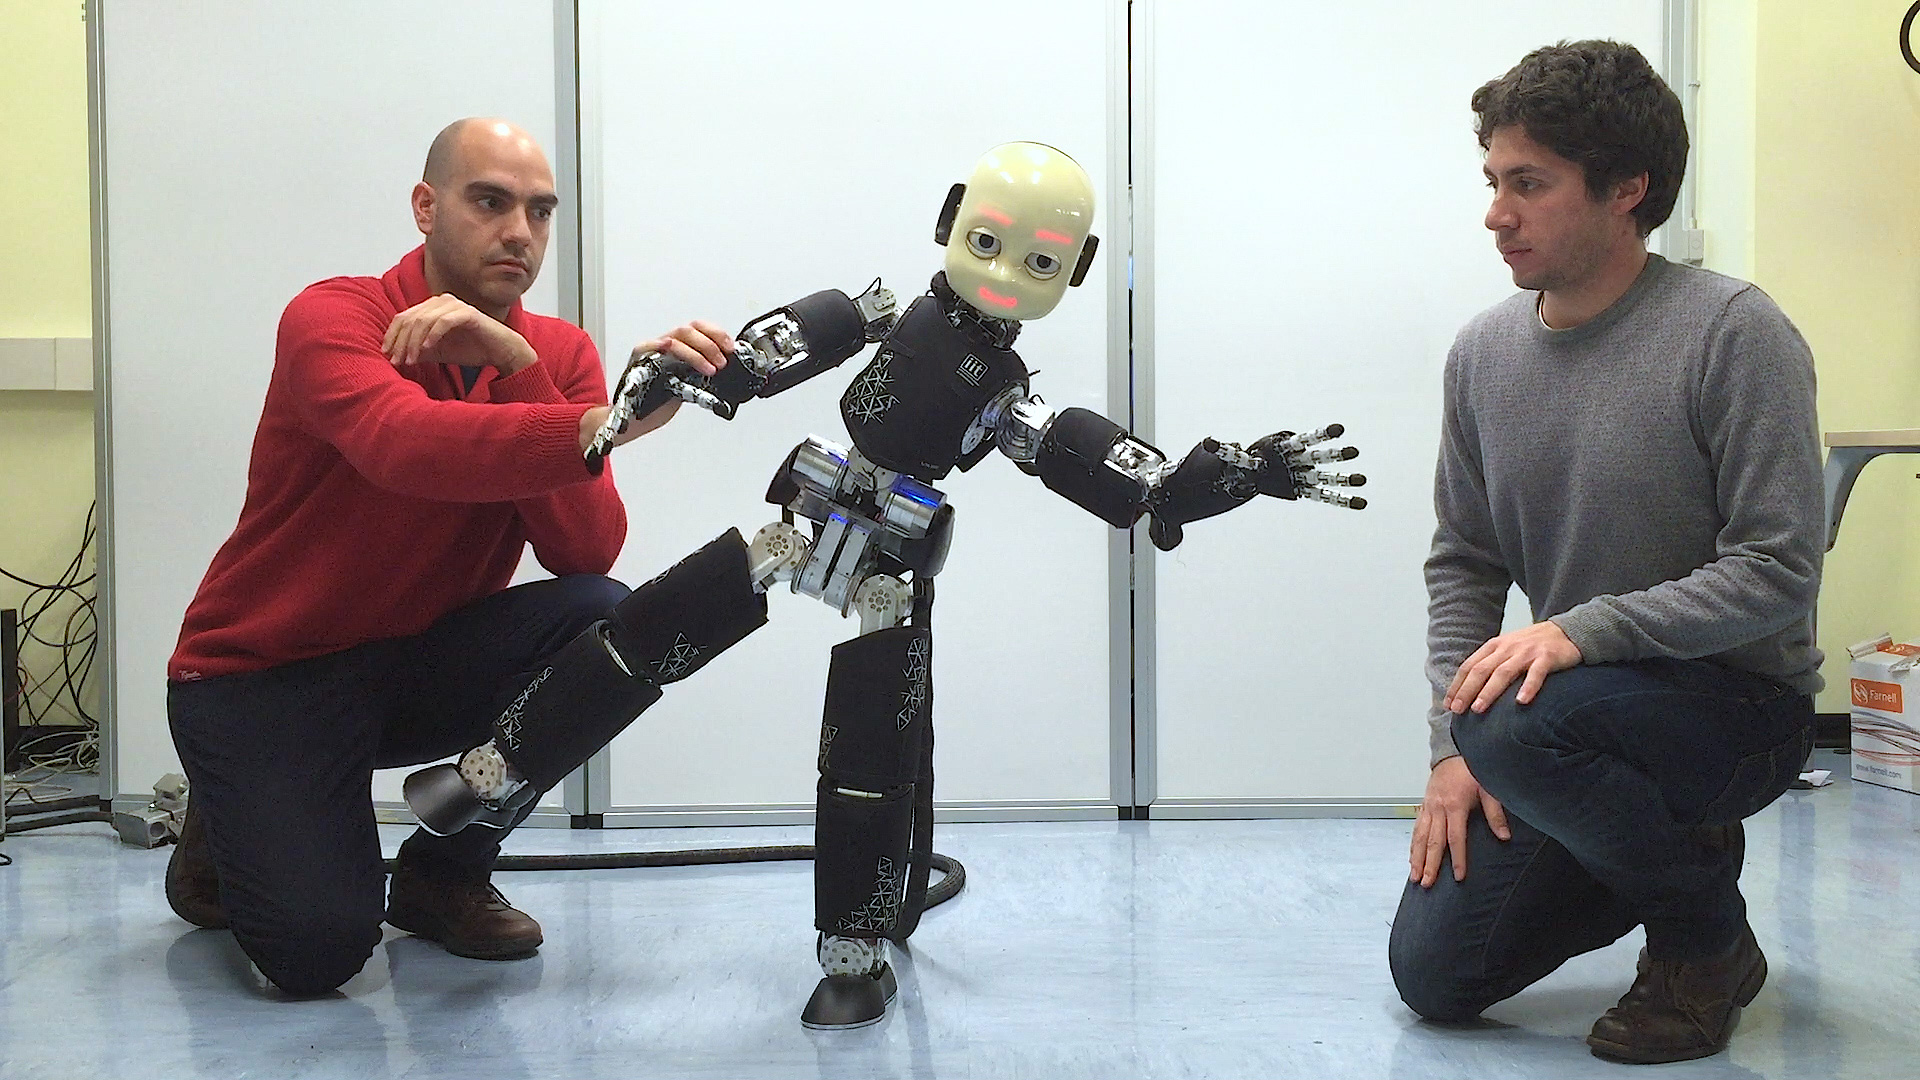
\includegraphics[width=0.65\columnwidth]{images/iCubInteractionOneFoot.jpg}
    \caption{A screen-shot of the one-foot balancing demo }
    \label{fig:oneFootBalnacing}
    }
\end{figure}

\begin{enumerate}
	\item Stabilization of the robot's momentum (expressed at the center-of-mass and with the inertial frame orientation), which is defined by
\begin{IEEEeqnarray}{RCL}
	\yesnumber
	H = \sum H_i = 
	\begin{pmatrix}
	m \dot{x} \\
	H_\omega
	\end{pmatrix},
	\nonumber
\end{IEEEeqnarray}
with $H_i$ the momentum of each link composing the multi-body system, $m$ the total mass of the robot, $x \in \mathbb{R}^3$ the position of the robot center-of-mass, and $H_\omega$ the angular momentum of the multi-body system. 

The control of the robot momentum is achieved assuming the contact wrenches as a virtual control input in the dynamics of $H$. For instance, assuming that the robot is balancing on two feet, two external wrenches $f_L \in \mathbb{R}^6 $ and $f_R \in \mathbb{R}^6$ act on the left and right foot, respectively. Then, one has
\begin{IEEEeqnarray}{RCL}
	\label{centroidalMomentumDyn}
	\yesnumber
	\dot{H} = mg +^c X_L f_L +^c X_R f_R = mg + 
	\begin{pmatrix}
	^c X_L && ^c X_R 
	\end{pmatrix}	
	f,
\end{IEEEeqnarray}
where $^c X_L,^c X_R \in \mathbb{R}^{6\times6}$ are two proper projection matrices, and $f := (f_L^\top,f_R^\top)^\top$.
Since $f$ is assumed to be a control input, one can choose it so that $\dot{H} = \dot{H}^*$, where  $\dot{H}^*$ ensures that $x \rightarrow x_d$ and $H_\omega \rightarrow 0$. Clearly, at this level, one is left with a six-dimensional redundancy of the control input. This redundancy is exploited to minimize joint torques. 
	\item In the null space of the above task, we want the robot to assume a desired joint configuration, while having also some compliance. This is achieved by means of a postural task at the joint torque level, which exploits a proportional-derivative plus gravity compensation control strategy for stabilizing a desired joint reference.
\end{enumerate}

The above control objectives can be formulated as follows. 

\begin{IEEEeqnarray}{RCL}
	\IEEEyesnumber
	\label{optTorque}
	f^* &=& \argmin_{f}  |\tau^*(f)| \IEEEyessubnumber  \\
		   &s.t.& \nonumber \\
		   &&Cf < b \IEEEyessubnumber  \label{frictionCones} \\
		   && \dot{H}(f) = \dot{H}^* \IEEEyessubnumber \label{centroidal} \\
		   &&\tau^*(f) = \argmin_{\tau}  |\tau(f) - \tau_0(f)| 	\label{optPost} 
  \\
		   	&& \quad s.t.  \nonumber \\
		   	&& \quad \quad \ \dot{J}(q,\nu)\nu + J(q)\dot{\nu} = 0
		    \IEEEyessubnumber 	\label{constraintsRigid} \\
		   	&& \quad \quad \ \dot{\nu} = M^{-1}(S\tau+J^\top(q) f - h(q,\nu)) \IEEEyessubnumber \label{acceleration} \\
		   && \quad \quad \ 	\tau_0 = \bar{h}-\bar{J}^{\top}_j f- K_p (q_j-q^{des}_j)- K_d (\dot{q}_j-\dot{q}^{des}_j) \IEEEyessubnumber
		   \yesnumber
\end{IEEEeqnarray}
For the sake of completeness, in the above optimization problem one has
\begin{IEEEeqnarray}{RCL}
	\IEEEyesnumber \\
	 H_d&:=&
\begin{pmatrix}
m\dot{x}_d \\
0
\end{pmatrix}	 \IEEEyesnumber \\
\tilde{H} &:=&H-H_d
\IEEEyessubnumber\\
	\dot{H}^* &=& \dot{H}_d - k_d\tilde{H} -k_p \int_0^t\tilde{H} ds
%	\begin{pmatrix}
%		m(\ddot{x}_d - k_p(x-x_d)-k_d(\dot{x}-\dot{x}_d)) \\
%		-k_\omega H_\omega -k_i \int_0^t  H_\omega ds
%	\end{pmatrix}	 
\IEEEyessubnumber\\
	\bar{h} &:=& h_j - M^\top_{bj}M^{-1}_b h_b \IEEEyessubnumber \\
	\bar{h} &:=& 
	\begin{pmatrix}
	h_b \\ h_j
	\end{pmatrix} =
	{C}(q, {\nu}) {\nu} + {G}(q), \quad h_b \in \mathbb{R}^6 \quad h_j \in \mathbb{R}^n
	 \IEEEyessubnumber \\
	\bar{J} &:=& J_j - J^{\top}_b M^{-1}_b M_{bj} \IEEEyessubnumber	\\
	M &=& 
	\begin{pmatrix}
		M_b && M_{bj} \\
		M^{\top}_{bj} && M_j
	\end{pmatrix}	 \quad M_b \in \mathbb{R}^{6\times 6}
	\quad M_{bj} \in \mathbb{R}^{6\times n}
	\quad M_b \in \mathbb{R}^{n\times n}\IEEEyessubnumber
\end{IEEEeqnarray}

Note that the additional constraint~\eqref{frictionCones} ensures that the desired contact wrenches $f$ belong to the associated friction cones. Once the optimum $f^*$ has been determined, the input torques $\tau$ are obtained by re-using the expression~\eqref{optPost}, i.e.
\begin{IEEEeqnarray}{RCL}
	\label{optTorqueFinal}
	\tau = \tau^*(f^*)
		   \yesnumber
\end{IEEEeqnarray}
By direct calculations one can verify that the solution to the problem~\eqref{optPost} is an affine function versus the desired wrenches $f$, i.e. 
$\tau^* = A(q,\nu)f + b(q,\nu),$
where $A \in \mathbb{R}^{n\times 12}$ and $b \in \mathbb{R}^{n}$ two proper matrices. 
This leads to the following simplification of the optimization problem 
\begin{IEEEeqnarray}{RCL}
	\label{optTorque2}
	\IEEEyesnumber
	f^* &=& \argmin_{f}  |\tau^*(f)|  \IEEEyessubnumber \\
		   &s.t.& \nonumber \\
		   &&Cf < b \IEEEyessubnumber  \label{frictionCones2} \\
		   && \dot{H}(f) = \dot{H}^* \IEEEyessubnumber \\
		   &&\tau^*(f) = A(q,\nu)f + b(q,\nu) \IEEEyessubnumber
		   \yesnumber
\end{IEEEeqnarray}
The above control algorithm has run at both review meetings of the CoDyCo project.

\subsection{Exploiting human-robot interaction  during standing-up motion: passivity based control} 
\begin{figure}
\centering
\begin{subfigure}{.32\textwidth}
  \centering
  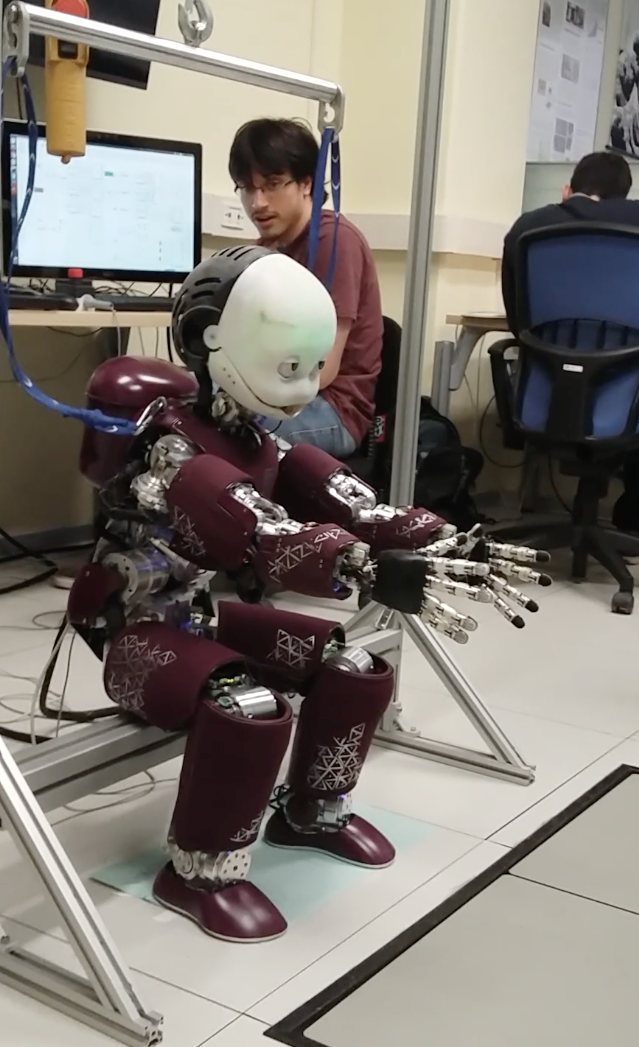
\includegraphics[width=.33\linewidth]{images/icubOnChair.jpg}
  \caption{iCub seating on a bar}
  \label{fig:sub1}
\end{subfigure}%
\begin{subfigure}{.34\textwidth}
  \centering
  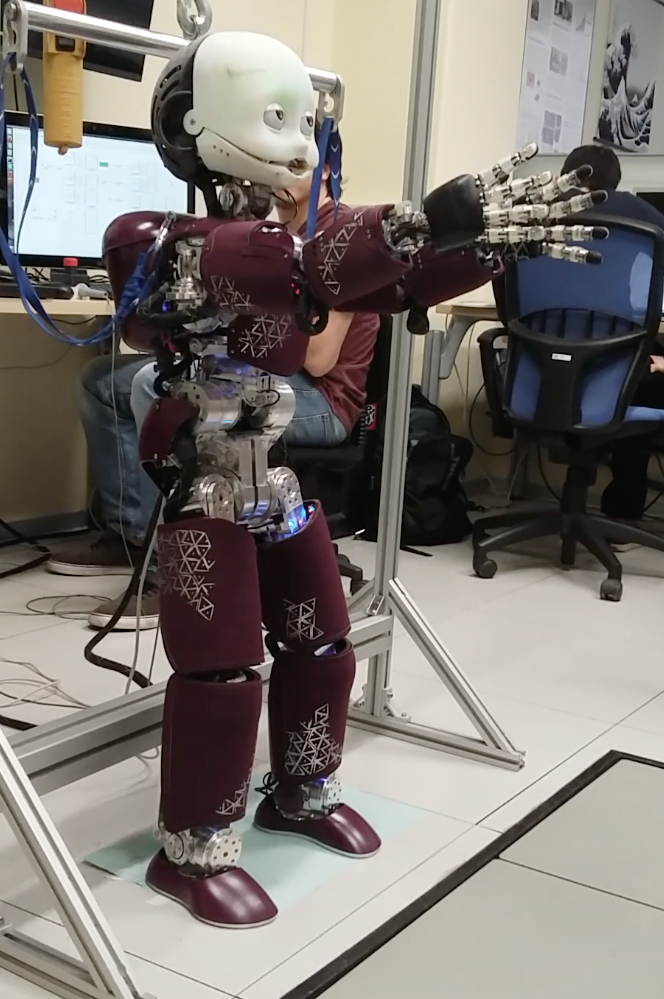
\includegraphics[width=.34\linewidth]{images/iCubUp.jpg}
  \caption{iCub standing on two feet }
  \label{fig:sub2}
\end{subfigure}
\begin{subfigure}{.33\textwidth}
  \centering
  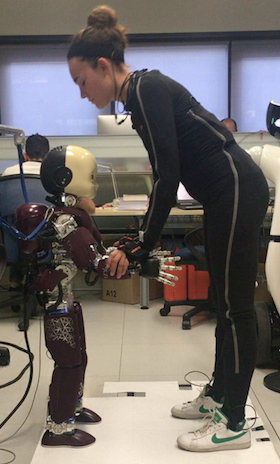
\includegraphics[width=.32\linewidth]{images/icubInteraction.jpg}
  \caption{iCub interacting with users}
  \label{fig:sub3}
\end{subfigure}
\caption{The standing up motion with and without user interaction}
\label{fig:standingUp}
\end{figure}


The controller recalled in the previous section implements on the robot the capacity of stabilising a desired trajectory for the  center-of-mass and a desired joint trajectory. Clearly, both these desired trajectories can be associated with a standing-up motion from the robot being seated on  thighs to the robot standing on two feet, see Figure~\ref{fig:sub1}-\ref{fig:sub2}. A finite state machine coordinates the transitions between these two different robot states by dictating the constraints acting on the system, which in turn characterise  the solutions to the optimisation problem~\eqref{optTorque}. Now, when a user interacts with the robot, it creates external forces on the mechanical system representing it, see Figure~\ref{fig:sub3}. These forces must be taken into account during the standing-up motion in order to make the robot robust against the external perturbations the user creates on the robot. 

Let $F_{ext} \in \mathbb{R}^{n+6}$ denote the torques produced by the external forces acting on the robot. Then,
 assuming that these torques can be measured by means of the force/torque sensors installed within the robot, a very simple way to take into account the external forces is to solve the optimisation problem~\eqref{optTorque} with the constraints~\eqref{centroidal} and~\eqref{acceleration} substituted by:
\begin{IEEEeqnarray}{RCL}
		   	\dot{H}&=&  mg + 
	\begin{pmatrix}
	^c X_L && ^c X_R 
	\end{pmatrix}	
	f + f_{ext}, \IEEEyessubnumber \label{centroidal1}  \\
 	 		\dot{\nu} &=& M^{-1}(S\tau+J^\top(q) f - h(q,\nu)+F_{ext}) \IEEEyessubnumber \label{acceleration1}, 
\end{IEEEeqnarray}
respectively. In the above equation, $f_{ext}\in \mathbb{R}^6$ is the effect of the external wrenches on the centroidal dynamic $\dot{H}$. One of the main problems due to the above approach is that the external wrenches applied on the robot would be completely canceled by the pure feedback linearisation controller associated with this strategy. The macroscopic effect of this cancellation is that if a user would like to \emph{help the robot stand up}, the robot motion would be invariant with respect to the help provided by the user since the effects of the external wrenches are canceled out: in fact, the closed loop dynamics does not depend upon it. So the main question now is:

\vspace{0.5cm}
\noindent
\emph{How can we synthesize a controller that implements the possibility for a user to help the robot lift up during the standing up motion?}
\vspace{0.5cm}

To answer this question, we have to focus on Eq.~\eqref{centroidal1}, and on the role of the fictitious control input $f$ to obtaining $\dot{H}(f) = \dot{H}^*$. First, recall that  $\dot{H}^*$, i.e.
\begin{IEEEeqnarray}{RCL}
	\dot{H}^* &=& \dot{H}_d - k_d\tilde{H} -k_p \int_0^t\tilde{H} ds \nonumber
\end{IEEEeqnarray}
renders the Lyapunov function 
\begin{IEEEeqnarray}{RCL}
	V &=& \frac{1}{2}|\tilde{H}|^2 + \frac{ k_p}{2} \left| \int_0^t\tilde{H} ds  \right | ^2 \label{eq:Lyapuv}
\end{IEEEeqnarray}
negative semi-definite, i.e.
\begin{IEEEeqnarray}{RCL}
	\dot{V} &=& -k_d|\tilde{H}|^2 \label{eq:LyapuvDer}.
\end{IEEEeqnarray}
The equation~\eqref{eq:LyapuvDer} stresses that  that an eventual help from a user to lift the robot up is useless: the rate of change of $V$ does not depend upon the external forces, so the standing up motion is invariant to the user interactions. The modification we propose here is based on a decomposition of the external force $f_{ext}$ that highlights the component of this external force that helps decrease the function $V$. More precisely, decompose the external force as follows:
\begin{IEEEeqnarray}{RCL}
	\label{forcedec}
	f_{ext} &=& \alpha\tilde{H}^\parallel + \beta \tilde{H}^\perp \IEEEyessubnumber \label{forcedec1} \\
	\tilde{H}^\parallel  &=&  \frac{\tilde{H}}{|\tilde{H}|}\IEEEyessubnumber \label{forcedec2}  \\
	\alpha &=& \frac{\tilde{H}^\top f_{ext} }{|\tilde{H}|}\IEEEyessubnumber \label{forcedec3}
\end{IEEEeqnarray}
Note that the scalars $\alpha$ and $\beta$ are the components of the external force $f_{ext}$ along and perpendicular to the momentum error $\tilde{H}$. Now, re-define $\dot{H}^*$ as follows 

\begin{equation}
\label{eq:newHStarDot}
  \dot{H}^* =
  \begin{cases}
    \dot{H}_d - k_d\tilde{H} -k_p \int_0^t\tilde{H} ds & \text{if }\quad  \alpha > 0
    \\
   \dot{H}_d - k_d\tilde{H} -k_p \int_0^t\tilde{H} ds +\alpha\tilde{H}^\parallel & \text{if }\quad  \alpha \leq 0
  \end{cases}
\end{equation}
and choose the control input $f$ such that 
\[ \dot{H}(f) = \dot{H}^*. \]
By computing the time derivative of~\eqref{eq:Lyapuv} along the system evolution~\eqref{centroidal1}-\eqref{forcedec}, one easily verifies that:
\begin{equation}
\label{eq:newHStarDot}
 \dot{V} =-k_d|\tilde{H}|^2 +
  \begin{cases}
   0 & \text{if }\quad  \alpha > 0
    \\
   \alpha|\tilde{H}| & \text{if }\quad  \alpha \leq 0
  \end{cases}
\end{equation}
The fact that when the external forces \emph{help} the robot stand up is encompassed in the right hand side of the above equation:  a negative $\alpha$, i.e. the external forces are in the direction of motion, make the Lyapunov function decrease faster.


\section{Conclusion}

In this deliverable, an overview of the work performed, within the framework of the CoDyCo project, on balancing with compliant contacts is provided. This work is the result of tasks T3.2, T3.3 and T5.3.

The adaptive approach described in \cite{liu_IROS2015} has the advantage of providing a way to accommodate compliant contacts without the need for a model. Its major disadvantage lies in the fact that it aims at reaching a state where, after a transient period, compliant contacts are fully compressed and can be used as rigid ones. Unfortunately, in highly compliant environment this is never the case and one actually has to balance with contact points that remain compliant. A second disadvantage is that the proposed algorithm tends to require  more forces from the most compliant contact points. This may be critical if the corresponding contacts corresponds to fragile surfaces which may break under high contact forces.\\

The two other proposed approaches \cite{AzadIROS2015}, \cite{deliverable53} assume that a model of the compliant contact is known. While the approach described in Deliverable~5.3 \cite{deliverable53} is less sensitive to the quality of the estimation of this model, the identification problem remains a complex one. At this stage estimation is performed off-line through a tedious procedure. In practical cases where the environment may not be known in advance, online estimation techniques would be needed. However, these methods are still to be developed, in a context  where estimating dynamic quantities (for example the floating-base state) for rigid multi-body systems remains a recent research topic \cite{nori2015simultaneous}, \cite{rotella2015humanoid}.


\newpage{}

\phantomsection
\bibliographystyle{IEEEtran}
% argument is your BibTeX string definitions and bibliography database(s)
\bibliography{IEEEabrv,D3.2}
\addcontentsline{toc}{section}{References}

\newpage{}
\begin{appendices}
\appendices



\end{appendices}




\end{document}

%%% Local Variables:
%%% mode: latex
%%% TeX-master: t
%%% save-place: t
%%% End:
